\chapter{Cascade system performance evaluation}
\section{System description}
In the cascade system, dish collectors are used to provide heat for Stirling engines and air-to-water heat exchanger. Trough collectors are used to provide heat for steam generating processes (preheating, evaporating and superheating) in the Rankine cycle. Figure~\ref{fig:System-1} shows the scheme sketch of the cascade system. In this system, hot air is produced by the dish collectors. High temperature (1073\,K) air is used to provide heat to Stirling cycle to get higher conversion efficiency, then the air is used to provide heat for air-to-water heat exchanger to use the lower temperature energy in Rankine cycle effectively. Besides, feed water of Rankine cycle is used to cool the Stirling engines to recycle the heat wasted conventionally. 
%Water is used as the working fluid of Rankine cycle, which is heated in the cold chamber of Stirling engines, preheater, evaporator, superheater, and air-to-water heat exchanger successively, and then expand in turbine, condense in condenser. Pumps are used to change the pressure of fluids. Stirling engines are used for power generation and cooled by feed water of the Rankine cycle. 

\noindent \begin{figure}[htbp]
\begin{center}
	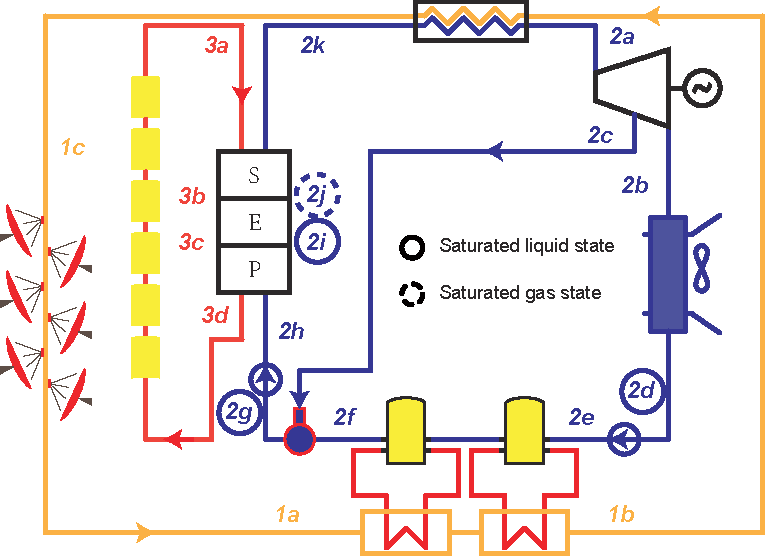
\includegraphics[width = 0.5\columnwidth]{fig/cascadeSystem}
	\caption{Sketch of the cascade system}
	\label{fig:System-1}
\end{center}
\end{figure}

State points of different fluids are marked on the sketch. The number indicates the type of the fluid, the letter indicates the state point of the fluid. State points with solid circle indicate saturated liquid states ($x = 0$\nomenclature{$x$}{Dryness fraction}), and with dotted circle indicates saturated gas states ($x = 1$). Figure~\ref{fig:T-s_Water2} shows the $T-s$ diagram of the water circuit in the cascade system. In this Rankine cycle, the heat provided in process $2e$-$2f$ comes from the Stirling engines, which increases the power of Rankine cycle. Figure~\ref{fig:HeatTransfer_Water-SEs} shows the heat transfer diagram of this process.

\noindent \begin{figure}[htbp]
\centering
	\begin{subfigure}[b]{0.4\columnwidth}
	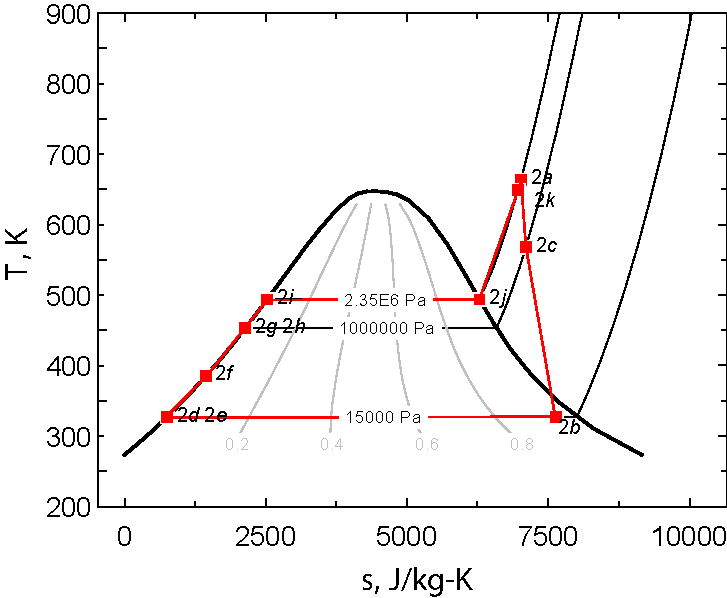
\includegraphics[width = \columnwidth]{fig/T-s_Water2}
	\caption{$T$-$s$ diagram of the water circuit}\label{fig:T-s_Water2}
	\end{subfigure}
	~
\begin{subfigure}[b]{0.4\columnwidth}
	\includegraphics[width = \columnwidth]{fig/HeatTransfer_Water-SEs}
	\caption{Diagram of process $2e$-$2f$}\label{fig:HeatTransfer_Water-SEs}
	\end{subfigure}
	
	\caption{Diagrams of water circuit and $2e$-$2f$ process}\label{fig:Diagrams$2e$-$2f$}
\end{figure}


%\noindent \begin{figure}[htbp]
%\begin{center}
%	\subfigure[$T-s$ diagram of the water circuit]{
%	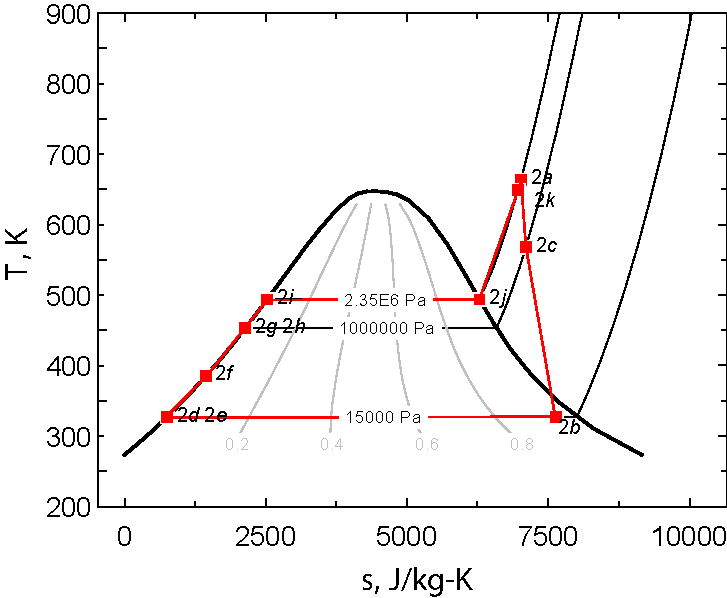
\includegraphics[width = 0.4\columnwidth]{fig/T-s_Water}
%	\caption{$T-s$ diagram of the water circuit}
%	\label{fig:T-s_Water}}
%	~\subfigure[Heat transfer diagram of process $2e$-$2f$]{
%	\includegraphics[width = 0.4\columnwidth]{fig/HeatTransfer_Water-SEs}
%	\caption{Heat transfer diagram of process $2e$-$2f$}
%	\label{fig:HeatTransfer_Water-SEs}}
%	\caption{Diagrams of water circuit and $2e$-$2f$ process}
%\end{center}
%\end{figure}

%\noindent \begin{figure}[htbp]
%\begin{center}
%	\includegraphics[width = 0.7\columnwidth]{./graphics/HeatTransfer_Water-SEs}
%	\caption{Heat transfer diagram of process $2e$-$2f$}
%	\label{fig:HeatTransfer_Water-SEs}
%\end{center}
%\end{figure}

To build the cascade system model, several simplifying assumptions are made:

\begin{itemize}
	\item Steady state at nominal load of the system is analysed.
	\item Pressure drop due to flow is negligible.
	\item The leak of working fluid in the pipes is neglected.
	\item Same isentropic efficiency of steam turbine with different loads and in different stages.
	\item Heat loss that occurs from the tube to the atmosphere is not considered.
	\item There is no heat loss to the environment for Stirling engines.
	\item Simple models are used of some processes and equipment.
	\item A symmetrical regenerator behavior is assumed so that a single effectiveness can be defined as $e = (T_R - T_L) /(T_H - T_L)$.~\cite{Formosa2010, Juhasz2010}
	\item A linear temperature profile across the regenerator exists, the mean effective temperature $T_{R} = (T_H-T_L) / \ln(T_H/T_L)$.~\cite{Der2007, Cavazzuti2012}
\end{itemize}

\section{Determination of system parameters}

\section{System simulation}

\section{Stand-alone system selection}

\noindent \begin{figure}[htbp]
\centering
	\begin{subfigure}[b]{0.63\columnwidth}
	\includegraphics[width = \columnwidth]{fig/Trough-s}
	\caption{Trough-Rankine system}\label{fig:TroughRankine}
	\end{subfigure}
	~
\begin{subfigure}[b]{0.266\columnwidth}
	\includegraphics[width = \columnwidth]{fig/Dish-s}
	\caption{Dish-Stirling system}\label{fig:DishStirling}
	\end{subfigure}
	
	\caption{Sketch of the stand-alone systems}\label{fig:Stand-alone-systems}
\end{figure}

%\noindent \begin{figure}[htbp]
%\begin{center}
%	\subfigure[Trough-Rankine system]{
%	\includegraphics[width = 0.45\columnwidth, angle = 0]{./graphics/Trough-s}}
%	\subfigure[Dish-Stirling system]{
%	\includegraphics[width = 0.19\columnwidth, angle = 0]{./graphics/Dish-s}}
%	\caption{Sketch of the stand-alone systems}
%	\label{fig:Stand-alone-systems}
%\end{center}
%\end{figure}

Figure~\ref{fig:Stand-alone-systems} shows the sketch of the stand-alone systems. These two stand-alone systems were developed for comparison. They use the same dish collectors and trough collectors with the same thermal efficiencies.

\subsection{Stand-alone trough-Rankine system}

Steam turbine has the same main parameters and isentropic efficiency with that of the cascade system. Working pressure of deaerator is the same of the cascade system. So parameters of state $2b,s$ and $2c,s$ in Figure~\ref{fig:Stand-alone-systems} of the steam turbine can be obtained by $\eta_{i,tb}= (h_{2a,s}-h_{2b,s})/(h_{2a,s}-h_{i,2b,s}) = (h_{2a,s}-h_{2c,s})/(h_{2a,s}-h_{i,2c,s})$.
%the following equations.

%\begin{equation}
%	\eta_{i,tb}=\frac{h_{2a,s}-h_{2b,s}}{h_{2a,s}-h_{i,2b,s}}
%\end{equation}
\nomenclature[S]{$s$}{Stand-alone systems}
%
%\begin{equation}
%	\eta_{i,tb}=\frac{h_{2a,s}-h_{2c,s}}{h_{2a,s}-h_{i,2c,s}}
%\end{equation}

The output power of steam turbine $P_{tb,s}=\left(1-y_{s}\right)\dot{m}_{2,s}\left(h_{2a,s}-h_{2b,s}\right)+y_{s}\dot{m}_{2,s}\left(h_{2a,s}-h_{2c,s}\right)$.

%\begin{equation}
%	P_{tb,s}=\left(1-y_{s}\right)\dot{m}_{2,s}\left(h_{2a,s}-h_{2b,s}\right)+y_{s}\dot{m}_{2,s}\left(h_{2a,s}-h_{2c,s}\right)
%\end{equation}

The output power of generator $P_{ge,s}=P_{tb,s}\eta_{ge}$.

%\begin{equation}
%	P_{ge,s}=P_{tb,s}\eta_{ge}
%\end{equation}

The total power of pumps $P_{pu,s}=\left(1-y_{s}\right)\dot{m}_{2,s}\left(h_{2e,s}-h_{2d,s}\right)+\dot{m}_{2,s}\left(h_{2g,s}-h_{2f,s}\right)$.

%\begin{equation}
%	P_{pu,s}=\left(1-y_{s}\right)\dot{m}_{2,s}\left(h_{2e,s}-h_{2d,s}\right)+\dot{m}_{2,s}\left(h_{2g,s}-h_{2f,s}\right)
%\end{equation}

Heat injected in the water circuit $Q_{2,s}=\dot{m}_{2,s}\left(h_{2a,s}-h_{2g,s}\right)$.

%\begin{equation}
%	Q_{2,s}=\dot{m}_{2,s}\left(h_{2a,s}-h_{2g,s}\right)
%\end{equation}

The generator efficiency is the same of that in the cascade system, and the efficiency of Rankine cycle can be expressed as $\eta_{rk,s}=(P_{tb,s}-P_{pu,s}/\eta_{ge})/Q_{2,s}$.

%\begin{equation}
%	\eta_{rk,s}=(P_{tb,s}-P_{pu,s}/\eta_{ge})/Q_{2,s}
%\end{equation}

\subsection{Stand-alone dish-Stirling system}

In the stand-alone dish-Stirling system, Stirling engines with the same number of dish collectors are directly put on the focuses of the dish collectors. Water is used for cooling the Stirling engines. $T_{H,s}$ is chosen to be equal to outlet temperature of air in dish receiver. $T_{L,s}$ is chosen to be 310 K, the default expansion temperature in Fraser's dissertation~\cite{Fraser2008} for the calculation of 4-95 NK\uppercase\expandafter{\romannumeral2} engine. $k$ and $\gamma$ are chosen the same value as that of the Stirling engines in the cascade system.

%\begin{equation}
%	\eta_{sea,s}=\dfrac{T_{H,s}-T_{L,s}}{T_{H,s}+\dfrac{1-e_{s}}{k-1}\cdot\dfrac{T_{H,s}-T_{L,s}}{\ln\gamma}}
%\end{equation}
%
%where, $T_{R,s}=\dfrac{T_{H,s}-T_{L,s}}{\ln(T_{H,s}/T_{L,s})}$ and $e_{s}=\dfrac{T_{R,s}-T_{L,s}}{T_{H,s}-T_{L,s}}$.
%
The power of Stirling engines $P_{sea,s}=n_{dc}A_{dc}I_r\eta_{dc}\eta_{sea,s}$.

%\begin{equation}
%	P_{sea,s}=n_{dc}A_{dc}I_r\eta_{dc}\eta_{sea,s}
%\end{equation}
\nomenclature{$n$}{Number of collectors}

\section{Comparison with stand-alone system}
\section{System analysis}